\documentclass[twoside,11pt,openright]{report}

\usepackage[utf8]{inputenc}
\usepackage[american]{babel}
\usepackage{a4}
\usepackage{latexsym}
\usepackage[numbers]{natbib}
%\usepackage[square,semicolon,sort,longnamesfirst]{natbib}
\usepackage{amssymb}
\usepackage{amsmath}
\usepackage{epsfig}
\usepackage{graphicx}
\usepackage[T1]{fontenc}
\usepackage{lmodern}
\usepackage{color}
\usepackage{datetime}
\usepackage{epstopdf} 

\renewcommand*\ttdefault{txtt}

\newcommand{\todo}[1]{{\color[rgb]{.5,0,0}\textbf{$\blacktriangleright$#1$\blacktriangleleft$}}}


% see http://imf.au.dk/system/latex/bog/

\begin{document}

%%%%%%%%%%%%%%%%%%%%%%%%%%%%%%%%%%%%%%%%%%%%%%%%%%%%%%%%%%%%%%%%%%%%%%%

\pagestyle{empty} 
\pagenumbering{roman} 
\vspace*{\fill}\noindent{\rule{\linewidth}{1mm}\\[4ex]
{\Huge\sf 2D Orthogonal Range Search}\\[2ex]
{\huge\sf Mads Ravn, 20071580}\\[2ex]
\noindent\rule{\linewidth}{1mm}\\[4ex]
\noindent{\Large\sf Master's Thesis, Computer Science\\[1ex] 
\monthname\ \the\year  \\[1ex] Advisor: Kasper Green Larsen\\[15ex]}\\[\fill]}

\epsfig{file=logo.eps}\clearpage

%%%%%%%%%%%%%%%%%%%%%%%%%%%%%%%%%%%%%%%%%%%%%%%%%%%%%%%%%%%%%%%%%%%%%%%

\pagestyle{plain}
\chapter*{Abstract}
\addcontentsline{toc}{chapter}{Abstract}

\todo{in English\dots}

\chapter*{Resum\'e}
\addcontentsline{toc}{chapter}{Resum\'e}

\todo{in Danish\dots}

\chapter*{Acknowledgements}
\addcontentsline{toc}{chapter}{Acknowledgments}

\todo{\dots}

\vspace{2ex}
\begin{flushright}
  \emph{Mads Ravn,}\\
  \emph{Aarhus, \today.}
\end{flushright}

\tableofcontents
\pagenumbering{arabic}
\setcounter{secnumdepth}{2}

%%%%%%%%%%%%%%%%%%%%%%%%%%%%%%%%%%%%%%%%%%%%%%%%%%%%%%%%%%%%%%%%%%%%%%%

\chapter{Introduction}
\label{ch:intro}
In an age where everybody is presented with the possibility of searching through a lot of data, for example ebay.com and bilzonen.dk, we are interested in fast queries with as little overhead space usage as possible. We want to do two-dimensional orthogonal range search in our database, which means we can select two axes on which we can select results between two points on each. We are essentially forming an axis-aligned rectangle and selecting all points which lie within it. \todo{Rewrite - Ellis style} \\

\noindent \textbf{Orthogonal Range Searching.} \emph{Orthogonal range searcing} is one of the most fundamental and well-studied problems in computational geometry. Even with extensive research over three decades a lot of questions remain. In this thesis we will focus on $2D$ orthogonal range searching: Given $n$ points from $\mathbb{R}^2$ we want to insert them into a data structure which will be able to efficiently report which $k$ points lie within a given query range $\mathbb{Q} \subseteq \mathbb{R}^2$. This query can be defined as two corners of a rectangle, the lower left corner and the upper right corner, seeing as the query range is orthogonal to the axes. \\

\noindent \textbf{Word RAM Model.} \todo{Skriv om Word RAM Model sammenlignet med de andre typer her}\\

\noindent \textbf{Rank Space Reduction.} Given $n$ points from a universe $U$, the rank of a given point is defined as the amount of points which preceed it in a sorted list. Given two points $a,b \in U: a \leq b$ \emph{iff} $rank(a) \leq rank(b)$. Expanding this concept to 2 dimensions we have a set $P$ of $n$ points on a $U \times U$ grid. We compute for the \emph{x-rank} $r_x$ for each point in $P$ by finding the rank of the x-coordinate amongst all the x-coordinates in $P$. The \emph{y-rank} $r_y$ finds the rank of y-coordinate amongst all of the y-coordinates in $P$. Using \emph{rank space reduction} on $P$ a new set $P^*$ is constructed where $(x,y) \in P$ is replaced by $(r_x(x), r_y(y) \in P^*$. Given a range query $q = [x_1, x_2] \times [y_1, y_2]$, a point $(x,y) \in P$ is found within $q$ \emph{iff} $(r_x(x), r_y(y))$ is found within $q^* = [r_x(x_1), r_x(x_2)] \times [r_y(y_1), r_y(y_2)]$. \todo{Noget med at deres ordered property remains intact.} Computing the set $P^*$ from $P$ using rank space reduction, $P^*$ is said to be in rank space. While the $n$ points could be represented by $\lg U$ bits in $P$, they can now be represented by $\lg n$ bits in $P^*$ with $\lg n \ll \lg U$ which saves memory. \todo{We have essentially created a mapping between \dots } \\

\noindent \textbf{Ball Inheritance Problem.} Given a perfect binary tree with $n$ leaves, we want to distribute $n$ labelled balls which appear in an ordered list at the root to the leaves in $\lg n$ steps. \todo{Rephrase}. The list of balls at a given node will inherited by its children with each child receiving the same amount of balls. Each level of the tree contains the same amount of balls. Eventually each ball reaches a leaf of the tree and each leaf will contain exactly one ball. The identity of a given ball is a node and the index of the ball in that nodes list. The true identity, the information the ball contains, only lies in the leaf. The \emph{ball-inheritance problem} is to track a ball from a given node to a leaf and report the identity of the leaf. \\

\noindent \textbf{Ball Inheritance.} Given a perfect binary tree with $n$ leaves and $n$ labelled balls at the root the idea is to distribute the balls from the root to the leaves. The balls at the root are contained in an ordered list and for each ball in a nodes list one of its children is picked to inherit the ball such that both children recieve the same amount of balls. Each level of the tree contains the same amount of balls, and at level $i$ each ball contains $2^i$ balls. Eventually each ball reaches a leaf of the tree and each leaf will contain exactly one ball. The identity of a given ball is a node and the index of the ball in that nodes list. The goal is to track a balls inheritance from a given node to a leaf and report the identity of the leaf. When refering to ball inheritance the words \emph{ball} or \emph{point} can be used interchangebly. \\


\noindent \textbf{Outline.} \\

\noindent \textbf{Notation.} The set of integers ${i, i+1, \dots, j-1, j}$ is denoted by $[i,j]$. When no base is explicitely given logarithm will have base $2$. $\epsilon$ is an arbitrary small constant. Given an array $A$, $A[i]$ denotes the entry with index $i$ in $A$ and $A[i,j]$ denotes the subarray containing the entries from $i$ to $j$ in $A$. Throughout the thesis the successor of $x$ will be meant as the first number which is greater or equal to $x$ - the same applies for predecessor of $x$.


%%%%%%%%%%%%%%%%%%%%%%%%%%%%%%%%%%%%%%%%%%%%%%%%%%%%%%%%%%%%%%%%%%%%%%%
\part{Theory}
\chapter{Related Work}

In this chapter the original work of \citet{chanetal} is presented followed by a simplification of their idea. This simplification serves two purposes: It will be easier to implement which will present a much cleaner code to read and it will be easier to execute since it has much less things to compute and look up. The theory behind a $kD$-tree will also be explained as it is the de facto standard of orthogonal range queries today and will be used to compare the practical results of the simplified model.

This simplified range searching is still theoritically faster than the kd-tree which is the standard range search used today. 

\section{kd-trees}

The current standard of range reporting is kd-trees. This technique will be used as a reference point when evaluting the results of the primary work in this thesis. With linear space it is optimal for range reporting on the RAM.

A kd-tree is constructed recursively: Given $n$ points, the median of the points with respect to x are found. All points which has an x-coordinate larger than the median goes to the right child, while points which has an x-coordinate smaller than the median, and the median point, goes to the left child. At the next level the points will be divived in a similar fashion, this time using the y-median and the y-coordinates instead. When dividing $n$ points, the median will be chosen as the $\lceil n/2 \rceil$-th smallest number \cite{compgeo}.
Switching back and forth between focussing on x or y is done at each level of the tree and this will be continued until a binary tree has been constructed with $n$ leaves.

The tree with $n$ points can be represented as flat array with $n$ entries. The $\lceil n/2 \rceil$-th element in the array is the root of the tree. And so forth.
 With this in mind, the entire tree can represented using a flat array with $n$ elements. 




\section{Original Range Searching}
\label{sect:original}
Utilizing the \emph{ball inheritance} concept \citeauthor{chanetal} propose a better solution for ranged search queries. With the same space complexity as the $kD$-tree, but lower query time. Theorem $2.1$ states that \emph{for any $2 \leq B \leq \lg^\epsilon n$, we can can solve $2$-d orthogonal range reporting in rank space with $\mathcal{O}(n \lg_B \lg n)$ space and $(1+k)\mathcal{O}(B \lg \lg n)$ query time.}

\subsection{Solving the ball-inheritance problem} 
\label{ssection:solving-ball}

Consider a perfect binary tree with $n$ leaves. At each level we use a bit vector $A[1..n]$ to indicate which of its children a ball is inherited by: If $A[i]$ is $0$ means that the ball with identity $i$ in that node was inherited by its left child and $1$ means that it was inherited by its right child. Given a node and an identity of a ball we can know calculate the balls identity in the node it is inherited by. The node can answer the query $rank(k) = \Sigma_{i \leq k} A[i]$. If a ball is inherited by the right child node its new identity at that node is $rank(i)$ because that is how many $1$s that preceeds it in the current node. If a ball is inherited by the left child node the new identity is then $i-rank(i)$. With this information it is possible to traverse down the tree following a ball from any given node to a leaf. There are n balls per level which is represented by a bit vector of size $n$ per level, so even though conceptually this bit vector is divided out amongst the nodes of that level, we can interchangebly think of a bit vector per level or a bit vector per node.\todo{Rephrase and replace} Each level in the tree uses $\mathcal{O}(n)$ bits to store the bit vectors. This adds up to $\mathcal{O}(n \lg n)$ bits, or $\mathcal{O}(n)$ words. This trivial solution to the ball-inheritance problem uses $\mathcal{O}(\lg n)$ query time. \\


A bit vector is an array with entries from the alphabet $\Sigma = {0,1}$, where each entry is used to indicate whether a left or right child has been chosen for ball inheritance. By expanding the alphabet we can point to the childrens children, $\Sigma = \{0,1,2,3\}$, the childrens childrens children, $\Sigma = \{0,1,2,3,4,5,6,7\}$, and so forth. Expanding the alphabet will use $\mathcal{O}(n \lg \Sigma)$ per level.


\subsection{Solving range reporting}
With a solution to the ball-inheritance problem, \citet{chanetal} proposes \textbf{Lemma 2.4} \emph{if the ball inheritance problem can be solved with space $S$ and query time $\tau$, $2$-d range reporting can be solved with space $\mathcal{O}(S+n)$ and query time $\mathcal{O}(\lg \lg n + (1+k) \dot \tau)$.}

Consider a perfect binary tree with $n$ leaves. The root contains $n$ points in $2$-d rank space. These $n$ balls are sorted by their y-rank and will keep this order all the way down the tree. If a node has $p$ points in its ball list, it will take $\frac{p}{2}$ points with the lowest x-rank and give to its left child and the rest to the right child. The actual coordinates of the balls are only stored at the leaves and we know that x-coordinates of the balls in the leaves are sorted from left to right - smallest to highest. Since we only store the actual xy-coordinates once this data structure uses linear space.

Having distributed the $n$ points from the root to the leaves, we require additional data structures in order to answer the range queries. We will use a succint data structure for the \emph{range minimum query}. Consider an array $A$ with $n$ comparable keys, the goal is to find the index of the minimum key in the subarray $A[j,i]$. \todo{Describe either the cartesian tree or reference 29}. For each node in the tree that is a right child we add a range minimum query structure. The indices are the y-rank and the keys are the x-rank that the given node contains. A range maximum query structure is added to the all the nodes which are left children. Each data structure uses an amount of bits linear of the size of the nodes ball list, making it $\mathcal{O}(n)$ bits per level of the tree and $\mathcal{O}(n \lg n)$ bits in all - i.e. $\mathcal{O}(n)$ words of space.

In order to use this new data structure to report points in the range of $[x_1, x_2] \times [y_1, y_2]$ we follow these steps:
\begin{enumerate}
  \item We find the rank space successor of $x_1$, $x^*_1$, and the rank space predecessor of $x_2$, $x^*_2$. We use these to find the lowest common ancestor of $x^*_1$ and $x^*_2$, $LCA(x^*_1, x^*_2)$. This is the lowest node in the tree containing at least all the points between $x_1$ and $x_2$. By knowing $x^*_1$ and $x^*_2$, finding the lowest common ancestor is a constant time operation. Given that points are in an array, we can use xor as our $LCA$ operation. \todo{rephrase}
  \item As in step $1$ where we found the rank space of the x-coordinates, we find the rank space coordinates of the y-coordinates, $y^*_1$ and $y^*_2$, inside the left and right child of $LCA(x^*_1, x^*_2)$.
  \item We now descend into the right child of $LCA(x^*_1, x^*_2)$ and use the range minimum query structure to the find the index $m$ (the y-rank) of the point with the smallest x-coordinate in the range $[y^*_1, y^*_2]$. Using the ball inheritance model we follow the path to the leaf to find the actual x-coordinate of the point. If the x-coordinate is smaller than $x_2$ we return the point as a result and recurse into the ranges of $[y^*_1, m-1]$ and $[m+1, y^*_2]$ in order to find more points. When this is done we apply the same concept to the left child of $LCA(x^*_1, x^*_2)$ using the range maximum query to find points above $x_1$.
\end{enumerate}

\todo{Insert figure to conceptually show we are working our way out from the inside}

In order to support the predecessor (and successor) search of step $2$ we are still missing a piece of the puzzle. We add a succint data structure for this purpose to some levels of the tree. Given a sorted array $A[1..n]$ of $\omega$-bit integers, we can support predecessor search queries in $\mathcal{O}(\lg \omega)$ time using $\mathcal{O}(n \lg \omega)$ space which supports oracle access to the entries in the array. \todo{reference}. The points in rank space of $\mathcal{O}(\lg n)$ bits will use $\mathcal{O}(n \lg \lg n)$ bits ($\omega = \lg n$) per level and $\mathcal{O}(n \lg n \lg \lg n)$ bits in all, which is $\mathcal{O}(n \lg \lg n)$ words. In order to reduce this to linear space we will only place this predecessor search structure at levels which are multiples of $\lg \lg n$. When using the predecessor search from $LCA(x^*_1, x^*_2)$ we go up to the closest ancestor to use its search structure. Searching takes $\mathcal{O}(\lg \lg n)$ time plus $\mathcal{O}(1)$ queries to the ball-inheritance structure. \todo{Why?}. Using the ball-inheritance structure we walk at most $\lg \lg n$ steps down while translating the ranks of $y_1$ and $y_2$ to the right and left child of $LCA(x^*_1, x^*_2)$. The reason why this structure is necessary for the y-ranks and not the x-ranks, is because of the way the points have been distributed in the ball-inheritance tree: From left to right, the leaves have x-rank $1,2,..n$ so we can easily locate a given range in x-dimension, but in order to keep track of the y-dimensional range we need to follow the balls down the ball-inheritance structure. Adding this structure to each $\lg \lg n$ level saves us from going all the way from the root down to the $LCA$. \todo{rephrase}

Step $3$ mainly requires the use of the ball-inheritance structure. The time to traverse this structure is dependend on the improvements we made in \ref{ssection:solving-ball}. An empty range will result in two queries, one query to each child of $LCA(x^*_1, x^*_2)$, otherwise it will not exceed twice the number of nodes beneath $LCA(x^*_1, x^*_2)$. \todo{Why?} \todo{Add time complexity when ball-inheritance improvements has been written}.

\section{Simplified Range Searching}

In this section we will describe a simplified model of the one mentioned in section \ref{sect:original}. It will mainly use the ball-inheritance structure. A predecessor search structure will be used a the root of the tree to find the rank space of two points, $(x_1,y_1)$ and $(x_2,y_2)$, delimiting the search range.
\todo{Nu hvor jeg lige har beskrevet den originale, hvor meget skal jeg så gå i detaljer med hvorfor vi gør tingene? Som f.eks. at have tingene i rank space}

The ball distribution part works the same way as it did in the original range searching by \citeauthor{chanetal}: Given a perfect tree with $n$ leaves, the $n$ points are sorted by their y-rank at the root. Distributing its balls, a node will give half of its points to each of its children: the smallest by x-rank to its left child and the highest by x-rank to its right child. The points in the two new lists will retain the same order as their parents.

Given a range query $q = [x_1, x_2] \times [y_1, y_2]$ we are going to find the rank successor of $x_1$ and $y_1$ and the rank predecessor of $x_2$ and $y_2$. \todo{Have we explained why this is?}. We call these $x^*_1, y^*_1, x^*_2$ and $y^*_2$. We use $x^*_1$ and $x^*_2$ to find the lowest common ancestor $LCA$ containing all the points between $x_1$ and $x_2$. We know the positions of the leaves containing $x^*_1$ and $x^*_2$ so we can traverse from the $LCA$ down to them both. Traversing to $x^*_1$, the first stop is the left child of the $LCA$. From here, each time a node selectes a left child as the path to $x^*_1$ we know that the subtree contained in the right child contains points between $x_1$ and $x_2$. Symmetrically, the same applies when going right from the $LCA$: Each time a node selects a right child on the path to $x^*_2$ the subtree contained in the left child contains points between $x_1$ and $x_2$. This concept is seen on figure \ref{fig:LCA}.

Traversing from the root to $LCA(x^*_1, x^*_2)$ and from the $LCA$ to the two leaves containing $x_1$ and $x_2$ requires $\mathcal{O}(\lg n)$ steps. Having this method to find the points within the range of $[x_1, x_2]$ we have now reduced the problem to a $1$-d range query. In order to keep track of which these points lie within the range of $[y_1, y_2]$ we will utilize the rank function from before, $rank(k) = \Sigma_{i \leq k} A[i]$, when working on a nodes ball-inheritance list $A$.

Using the bit vector to keep track of which range of points lies within the range of $[y_1, y_2]$, we keep updating this range to fit the children of the node. Using $0$ to indicate a point going to the left child and $1$ to indicate a point going to the right child, the new start- and stop-position in the left child is $start-rank(start)$ and $stop-rank(stop)$ and in the right child $rank(start)$ and $rank(stop)$. \todo{Insert figure about bit vectors dividing}


This is exactly the reason why the points are sorted by their y-rank at the root and keep this order: The property of y-range in the bit vectors need to be retained for this to work. \todo{Example or figure of the transitive property}

We continue this walk down the tree while updating the start-stop-positions of the bit vectors in the nodes until the leaves are reached or until an entire subtree can either be fully included or fully excluded. 

In order to make the rank query a constant time query, we create a partial rank sum list of the bit vector. This list contains the sum of the rank from $0$ to $i*\alpha$, where $\alpha$ is some constant. Using this partial rank sum list we can find the look up $rank(i*\alpha)$ and add the rank of the at most $\alpha$ next bits. Looking up the rank thusly takes $\mathcal{O}(1)$ time and requires $\mathcal{O}(n)$ space.

The actual coordinates of the points are only stored at the leaves which then takes up $\mathcal{O}(n)$ space. The rest of the tree only contains $\lg n$ levels of bit vectors of $n$ bits taking $\mathcal{O}(n \lg n)$ bits, $\mathcal{O}(n)$ words. Looking up the rank-space predecessor and successor of $x_1, x_2, y_1$ and $y_2$ using a simple binary search requires $\mathcal{O}(n)$ space and $\mathcal{O}(\lg n)$ time. Walking from the root to the $LCA$ requires $\lg n$ steps and $(1+k)\mathcal{O}(\lg n)$ \todo{Still pending improvements from section (improvements)} time where $k$ is the amount of results reported.

\begin{figure}[p]
    \centering
    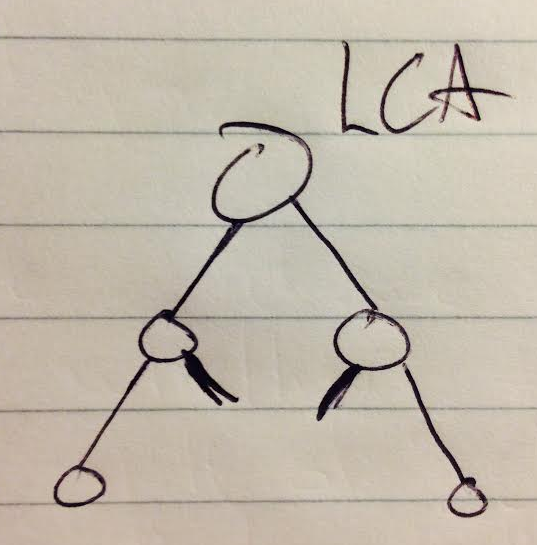
\includegraphics[width=0.8\textwidth]{pictures/LCA.png}
    \caption{Traversing left from the LCA, each right subtree contains x-coordinates between $x_1$ and $x_2$. Traversing right from the LCA the same holds for left subtrees.}
    \label{fig:LCA}
\end{figure}

\chapter{\todo{\dots}}
\label{ch:main}

%% \todo{example of a citation to primary literature: \citeA{lazypropagation2010},

%%%%%%%%%%%%%%%%%%%%%%%%%%%%%%%%%%%%%%%%%%%%%%%%%%%%%%%%%%%%%%%%%%%%%%%

\chapter{Conclusion}
\label{ch:conclusion}

\todo{\dots}

%%%%%%%%%%%%%%%%%%%%%%%%%%%%%%%%%%%%%%%%%%%%%%%%%%%%%%%%%%%%%%%%%%%%%%%

\addcontentsline{toc}{chapter}{Primary Bibliography}
\bibliographystyle{plainnat} 
\bibliography{refs}

\end{document}

